\section{}
%obvious one - derive time difference equations and then follow this through to finding some tones?
%quite easy but whatever

%picture of first order modulator
\begin{figure}
    \begin{center}
    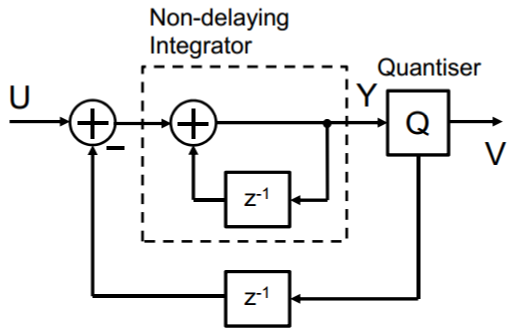
\includegraphics[width=0.8\textwidth]{firstorder.png}
    \caption{A first order modulator diagram.}
    \label{fig:firstorder}
    \end{center}
\end{figure}

    \subsection{}
    %find the time difference equations
    Express the modulator shown in figure \ref{fig:firstorder} in terms of time difference equations.
    
    \subsection{}
    \label{B2:2}
    %create a tone
    What is the period of the tone produced by a DC input of $\frac{2}{5}$?
    How many 1s and how many 0s does it contain?

    \subsection{}
    %FFT it
    Sketch a magnitude DFT of the tone in section \ref{B2:2}.

    \subsection{}
    %final part should involve multi-bit feedback and the tones produced with DWA
    If there were a 4 bit DWA DAC applied in this design with poorly matched components, what would you expected the period of the tones produced by it to be?

    %should double check this answer once I put it here
